\documentclass[12pt, twoside]{article}
\usepackage[letterpaper, margin=1in, headsep=0.5in]{geometry}
\usepackage[english]{babel}
\usepackage[utf8]{inputenc}
\usepackage{amsmath}
\usepackage{amsfonts}
\usepackage{amssymb}
\usepackage{tikz}
%\usetikzlibrary{quotes, angles}

\usepackage{graphicx}
\usepackage{enumitem}
\usepackage{multicol}

\usepackage{fancyhdr}
\pagestyle{fancy}
\fancyhf{}
\renewcommand{\headrulewidth}{0pt} % disable the underline of the header

\fancyhead[RE]{\thepage}
\fancyhead[RO]{\thepage \\ Name: \hspace{3cm}}
\fancyhead[L]{BECA / Dr. Huson / 10th Grade Geometry\\* 7 June 2019}

\begin{document}
\subsubsection*{13-6 Homework: Transformations, symmetry}
 \begin{enumerate}


  \item After a dilation with center $(0,0)$, the image of $\overline{RS}$ is $\overline{R'S'}$. If $RS=6.5$ and $R'S'=24$, find the scale factor of this dilation. \vspace{2.5cm}

  \item What series of transformations map $\triangle ABC$ onto $\triangle DEF$, shown below? Fully specify the transformations.
    \begin{center}
      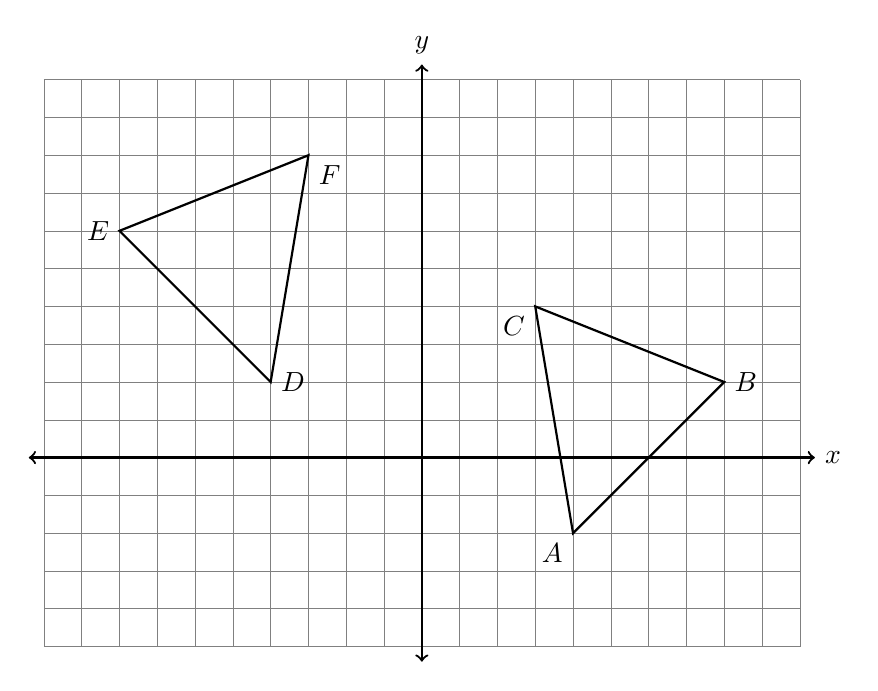
\begin{tikzpicture}[scale=.48]
        \draw [help lines] (-10,-5) grid (10,10);
        \draw [thick, <->] (-10.4,0) -- (10.4,0) node [right] {$x$};
        \draw [thick, <->] (0,-5.4)--(0,10.4) node [above] {$y$};
        \draw [thick]
          (4,-2) node[below left] {$A$}--
          (8,2) node[right] {$B$}--
          (3,4) node[below left] {$C$}--cycle;
        \draw [thick]
          (-4,2) node[right] {$D$}--
          (-8,6) node[left] {$E$}--
          (-3,8) node[below right] {$F$}--cycle;
      \end{tikzpicture}
    \end{center}
      \vspace{2cm}

  \item A translation maps $A(2,4) \rightarrow A'(-2,6)$. What is the image of $B(-1,5)$ under the same translation?  \vspace{1.5cm}

  \item What is the equation of a line resulting when the line $y=\frac{2}{3}x+3$ is dilated by a factor of 2 centered at the origin?

\newpage
  \item In the diagram below, $\triangle ABC$ with sides of 10, 12, and 11, is mapped onto $\triangle DEF$ after a clockwise rotation of $90^\circ$ about point $P$.
      \begin{center}
        \begin{tikzpicture}[scale=.6]
        \fill (0,0) circle[radius=0.1] node[right]{$P$};
          \draw [thick]
          (-2,1) node[below left] {$A$}--
          (-7,2) node[left] {$B$}--
          (-4,5) node[above right] {$C$}--cycle;
            \node at (-5,1.5)[below]{10};
            \node at (-6,4){12};
            \node at (-2.5,3.5){11};
            \node at (6,5.5){$2x+4$};
          \draw [thick]
          (1,2) node[left] {$D$}--
          (2,7) node[above] {$E$}--
          (5,4) node[right] {$F$}--cycle;
        \end{tikzpicture}
      \end{center}
    If $EF=2x+4$, what is the value of $x$? \vspace{3.5cm}

  \item The vertices of $\triangle JKL$ have the coordinates $J(-4,-2)$, $K(4,0)$, and $L(-2,4)$, as shown. \\[0.25cm]
    Apply a dilation to $\triangle JKL \rightarrow \triangle J'K'L'$, centered on $(2,2)$ with a scale factor $k=1.5$. Draw the image $\triangle J'K'L'$ on the set of axes below, labeling the vertices.
    \begin{center}
      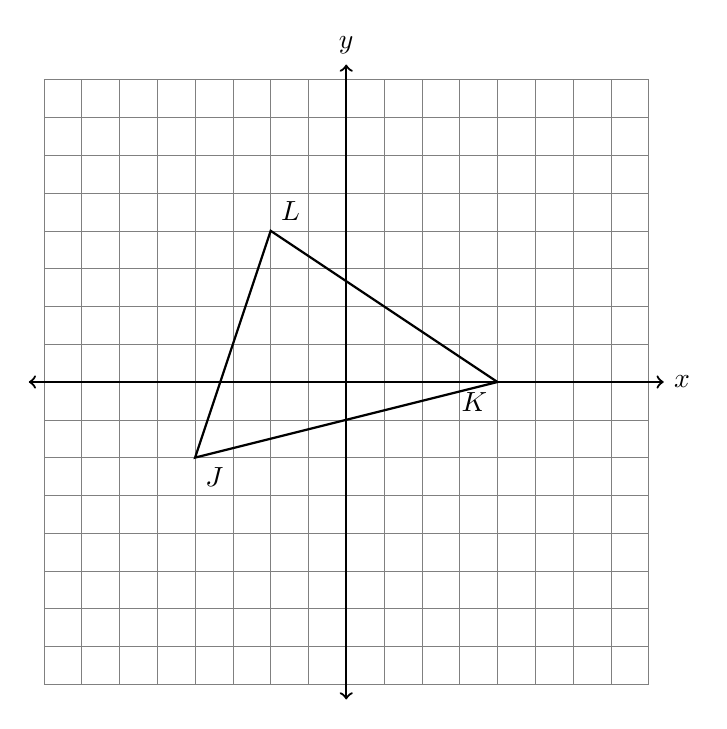
\begin{tikzpicture}[scale=.48]
        \draw [help lines] (-8,-8) grid (8,8);
        \draw [thick, <->] (-8.4,0) -- (8.4,0) node [right] {$x$};
        \draw [thick, <->] (0,-8.4)--(0,8.4) node [above] {$y$};
        \draw [thick]
        (-4,-2) node[below right] {$J$}--
        (4,0) node[below left] {$K$}--
        (-2,4) node[above right] {$L$}--
        cycle;
      \end{tikzpicture}
    \end{center}

\newpage

 \begin{multicols}{2} [\item Circle YES or NO to indicate whether the given transformation maps the hexagon onto itself.] %$ABCDEF$
 \vspace{0.5cm}
  \begin{enumerate}
    \item Yes \quad No \quad A rotation of $120^\circ$ counterclockwise around point $D$.
     \item Yes \quad No \quad A reflection over $\overleftrightarrow{AE}$
     \item Yes \quad No \quad A reflection over a line through the midpoints of  $\overline{BC}$ and $\overline{EF}$.
     \item Yes \quad No \quad A rotation of $60^\circ$ clockwise around the hexagon's center.
     \end{enumerate}
   \begin{center}
       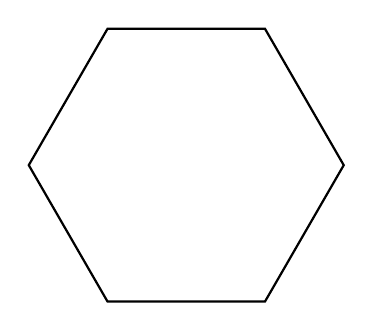
\begin{tikzpicture}%[scale=.48]
         \draw [thick]
         (0:2)--%  node[right] {$A$}--
         (60:2)--%  node[above right] {$B$}--
         (120:2)--%  node[above left] {$C$} --
         (180:2)--%  node[left] {$D$}--
         (240:2)--%  node[left] {$E$}--
         (300:2) --cycle;% node[right] {$F$}--cycle;
       \end{tikzpicture}
     \end{center}
   \end{multicols} \vspace{0.5cm}

  \item The $\triangle ABC$ is reflected across $l$ to yield $\triangle A'B'C'$. $AB=3x+4$, $A'B'=5x-10$, and $BC=4x+12$. Find the length $B'C'$. %\vspace{2cm}
      \begin{center}
      \begin{tikzpicture}[scale=.8]
        \draw [dashed, <->] (-1,-1)--(7,7) node[below right]{$l$};
        \draw [thick]
        (5,-1) node[below right] {$A$}--
        (8,2) node[right] {$B$}--
        (1,0) node[below left] {$C$}--cycle;
        \draw [thick]
        (-1,5) node[left] {$A'$}--
        (2,8) node[below right] {$B'$}--
        (0,1) node[below left] {$C'$}--cycle;
      \end{tikzpicture}
    \end{center} \vspace{2cm}

\newpage
 \item The figure shows a rectangle (not a square).
   \begin{center}
     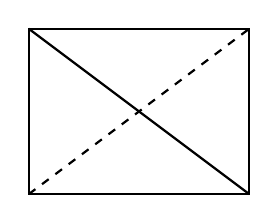
\begin{tikzpicture}[scale=0.7]
       \coordinate (A) at (0, 0); %[label=above left:$P$]
       \coordinate (B) at (4, 0);
       \coordinate (C) at (4, 3);
       \coordinate (D) at (0, 3);
       \draw [thick] (A)--(B)--(C)--(D)--cycle;
       \draw [thick, dashed] (A)--(C);
       \draw [thick] (B)--(D);
       %\draw [thick, xshift=2cm, yshift=2.5cm] (85:3);
     \end{tikzpicture}
   \end{center}
   Which transformations carries the rectangle onto itself? Mark each True or False.
     \begin{enumerate}
       \item A reflection over the solid diagonal \hfill True \quad False
       \item A reflection over the dashed diagonal \hfill True \quad False
       \item A clockwise rotation of $90^\circ$ about the intersection of the diagonals \hfill True \quad False
       \item A clockwise rotation of $180^\circ$ about the intersection of the diagonals \hfill True \quad False
     \end{enumerate}
     \vspace{1cm}

   \item The grid shows $\triangle ABC$ and $\triangle DEF$.
     \begin{center}
       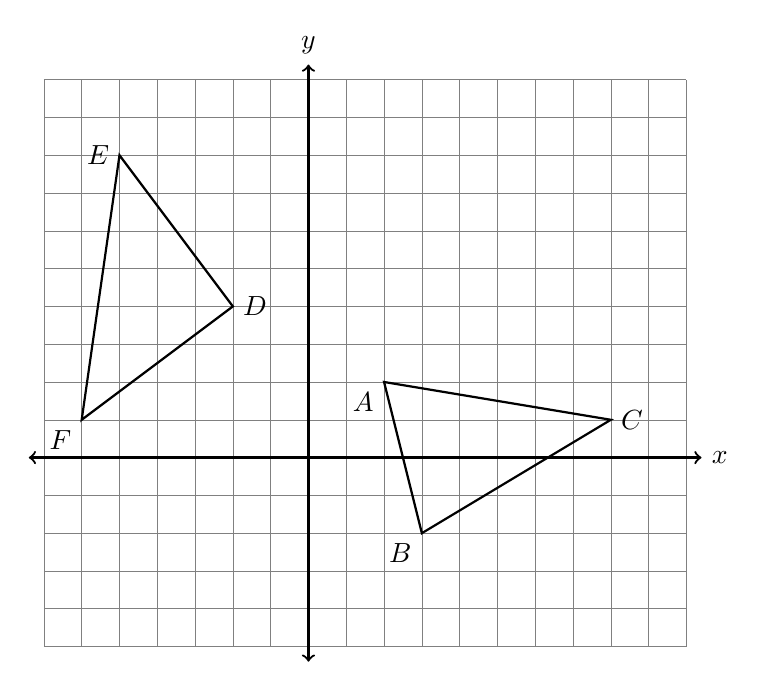
\begin{tikzpicture}[scale=.48]
         \draw [help lines] (-7,-5) grid (10,10);
         \draw [thick, <->] (-7.4,0) -- (10.4,0) node [right] {$x$};
         \draw [thick, <->] (0,-5.4)--(0,10.4) node [above] {$y$};
         \draw [thick]
           (3,-2) node[below left] {$B$}--
           (8,1) node[right] {$C$}--
           (2,2) node[below left] {$A$}--cycle;
         \draw [thick]
           (-2,4) node[right] {$D$}--
           (-5,8) node[left] {$E$}--
           (-6,1) node[below left] {$F$}--cycle;
       \end{tikzpicture}
     \end{center}
     Let $\triangle A'B'C'$ be the image of $\triangle ABC$ after a rotation about point $A$. Determine and state the location of $B'$ if the location of point $C'$ is $(3,8)$. Explain your answer, supported by stating the transformation applied.

 \newpage

  \item What is the smallest non-zero angle of rotation about its center that would map the pentagon onto itself? \vspace{0.25cm} %$ABCDE$
  \begin{center}
     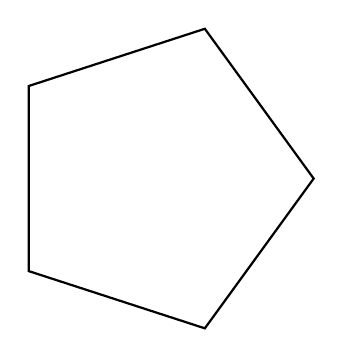
\begin{tikzpicture}%[scale=.48]
       \draw [thick]
       (0:2)--% node[right] {$A$}--
       (72:2)--% node[above right] {$B$}--
       (144:2)--% node[above left] {$C$} --
       (216:2)--% node[left] {$D$}--
       (288:2)--cycle;% node[right] {$E$}--cycle;
     \end{tikzpicture}
   \end{center} \vspace{0.5cm}

  \item What is the center and radius of the circle $(x+1)^2+(y-1)^2=16$? \vspace{2cm}

  \item Write down the equation of a circle with center $(3,5)$ and radius 8. \vspace{2cm}

  \item Expand the binomials and collect the fixed terms of the circle  $(x+2)^2+(y+1)^2=9$ \vspace{4cm}

  \item Which of these circles are larger, or are they the same size?
    \begin{enumerate}
      \item $(x-5)^2+(y+11)^2=4$
      \item $x^2+4x+y^2+2y=4$
    \end{enumerate}

\newpage
  \item Determine and state the transformation or sequence of transformations  applied to $\triangle ABC$, mapping it onto $\triangle PQR$, as shown.
   \begin{center}
       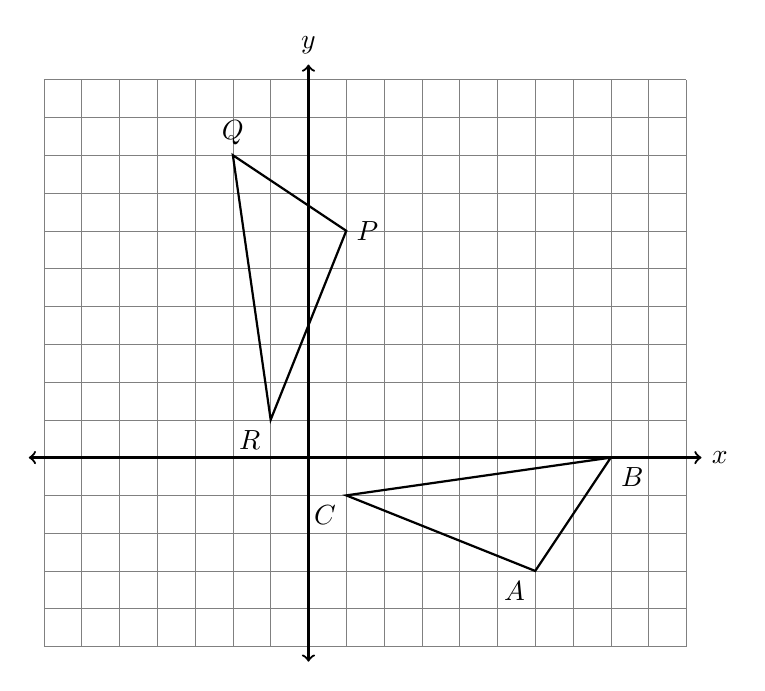
\begin{tikzpicture}[scale=.48]
         \draw [help lines] (-7,-5) grid (10,10);
         \draw [thick, <->] (-7.4,0) -- (10.4,0) node [right] {$x$};
         \draw [thick, <->] (0,-5.4)--(0,10.4) node [above] {$y$};

         \draw [thick]
         (6,-3) node[below left] {$A$}--
         (8,0) node[below right] {$B$}--
         (1,-1) node[below left] {$C$}--cycle;

         \draw [thick]
         (1,6) node[right] {$P$}--
         (-2,8) node[above] {$Q$}--
         (-1,1) node[below left] {$R$}--cycle;
       \end{tikzpicture}
     \end{center}
\vspace{2cm}

   \item Given parallelogram $ABCD$ with $m\angle A=65^\circ$, $AB=8$, and $BC=12$. Find the value of each angle measure or side length.
     \begin{enumerate}
       \item $m\angle B=$\vspace{0.5cm}
       \item $m\angle C=$\vspace{0.5cm}
       \item $m\angle D=$\vspace{0.5cm}
       \item $CD=$ \vspace{0.5cm}
       \item $AD=$ \vspace{0.5cm}
     \end{enumerate}

  \item Circle Always, Sometimes, Never, as applies.
    \begin{enumerate}
      \item Always \quad Sometimes \quad  Never \quad Opposite sides or a parallelogram are congruent.
      \item Always \quad Sometimes \quad  Never \quad Diagonals of a parallelogram are perpendicular.
      \item Always \quad Sometimes \quad  Never \quad All four sides of a trapezoid are congruent.
      \item Always \quad Sometimes \quad  Never \quad All four angles of a rhombus are congruent.
    \end{enumerate}

\end{enumerate}
\end{document}
